% Extensión estimada: 4.5--5 páginas (catorce párrafos, dos tablas, tres figuras y un fragmento de texto).
% Fuentes: conteos propios sobre Codigo/data/raw/HAM10000/HAM10000_metadata, Codigo/data/splits/ham10000_splits.json
% y ham10000_splits_lesion.json (solo lectura, 2026-10-11); Codigo/outputs/results/leakage_analysis.json;
% Codigo/scripts/make_lesion_disjoint_split.py; Codigo/scripts/prepare_data.py (splits de SkinCaRe);
% Codigo/data/splits/mmskin_splits.json, hiba_splits.json, skincare_*_splits.json. Figuras de HAM10000 generadas con
% Codigo/scripts/plot_ham_dataset_figs.py. Papers en Papers/derma/ (SkinCaRe, MM-Skin, HIBA, Derm1M).
% Claves: tschandl2018ham10000, shen2025skincare, groh2021neural, daneshjou2022disparities, daneshjou2022skincon,
% zeng2025mmskin, riccilara2023dataset, yan2025derm1miccv.
% Revisión del autor del 18/10/2026: menos cifras en el texto; los conteos completos quedan en tablas y figuras.
\section{Conjuntos de datos}
\label{sec:met_datasets}

El trabajo usa cinco conjuntos de datos de dermatología, que se diferencian por la modalidad de sus imágenes y por
el tipo de anotación que acompaña a cada una. \emph{HAM10000} reúne imágenes dermatoscópicas con un diagnóstico
confirmado y sin texto. \emph{SkinCaRe} y \emph{MM-Skin}, en cambio, asocian cada imagen a un texto clínico escrito
por dermatólogos, por un modelo de lenguaje o tomado de libros de dermatología. \emph{HIBA} aporta imágenes
dermatoscópicas y clínicas de un hospital argentino, y \emph{Derm1M} es un corpus de más de un millón de pares
imagen--texto. La Tabla~\ref{tab:met_conjuntos} resume, para cada uno, la modalidad, el tamaño, el uso en el trabajo y
el origen del texto de referencia.

Cada conjunto cumple un papel distinto en la experimentación, según sirva para entrenar, para evaluar o solo de forma
indirecta. \emph{HAM10000} es el único etiquetado con las siete categorías de la tarea, de modo que con él se entrenan
los clasificadores, se eligen sus configuraciones en validación y se evalúan en prueba todos los modelos de
clasificación y el \emph{pipeline}. Por esa razón es el conjunto central del trabajo, y sus propiedades, que se
analizan a continuación, determinan cómo se parte y con qué métricas se evalúa. \emph{SkinCaRe}, en cambio, se usa
para entrenar a los generadores de reportes, y \emph{MM-Skin}, para evaluarlos contra un texto de referencia.
\emph{HIBA} se usa solo como prueba externa, para comprobar si los clasificadores mantienen su desempeño en otra
población. Por último, \emph{Derm1M} no se usa de forma directa: es el conjunto con el que sus autores preentrenaron
DermLIP, uno de los modelos de la Sección~\ref{sec:met_clasif_vlm}.

\begin{table}[H]
    \centering
    \small
    \caption{Conjuntos de datos: modalidad, tamaño, uso en el trabajo y origen del texto de referencia.}
    \label{tab:met_conjuntos}
    \begin{tabularx}{\textwidth}{@{}>{\raggedright\arraybackslash}p{1.8cm}
        >{\raggedright\arraybackslash}p{2.5cm} >{\raggedright\arraybackslash}p{2.2cm}
        >{\raggedright\arraybackslash\hspace{0pt}}p{2.4cm} >{\raggedright\arraybackslash\hspace{0pt}}X@{}}
        \toprule
        \textbf{Conjunto} & \textbf{Modalidad} & \textbf{Tamaño} & \textbf{Uso} & \textbf{Origen del texto de referencia} \\
        \midrule
        \emph{HAM10000} & Dermatoscópica & 10\,015 imágenes; 7\,470 lesiones
            & Clasificación (entrenamiento, validación y prueba)
            & Sin texto; etiqueta confirmada por histopatología, seguimiento, consenso o microscopía confocal \\
        \filasep
        \emph{SkinCAP} (\emph{SkinCaRe}) & Clínica (fotografía) & 3\,561 imágenes
            & Entrenamiento de los generadores
            & Descripciones de cuatro dermatólogos, escritas en chino y traducidas al inglés \\
        \filasep
        \emph{SkinCoT} (\emph{SkinCaRe}) & Clínica (fotografía) & 3\,041 imágenes
            & Entrenamiento de los generadores; su prueba, evaluación con referencia
            & Razonamiento escrito por un modelo de lenguaje con la etiqueta a la vista y revisado por dermatólogos \\
        \filasep
        \emph{MM-Skin} & Clínica, dermatoscópica y patológica
            & 11\,039 imágenes; 9\,369 pares imagen--texto
            & Evaluación de los generadores con referencia
            & Descripciones de libros de texto de dermatología \\
        \filasep
        \emph{HIBA} & Dermatoscópica y clínica
            & 1\,616 imágenes; 1\,246 lesiones
            & Evaluación externa de los clasificadores (solo prueba)
            & Diagnóstico de dermatólogos del hospital, con histopatología en las lesiones extirpadas \\
        \filasep
        \emph{Derm1M} & Dermatoscópica y clínica & 1\,029\,761 pares imagen--texto
            & Preentrenamiento de DermLIP por sus autores (no se usa de forma directa)
            & Fuentes web, educativas y bases públicas; texto procesado con un \gls{llm} \\
        \bottomrule
    \end{tabularx}
\end{table}

\subsection{HAM10000: composición y análisis exploratorio}
\label{sec:met_ham}

\emph{HAM10000} contiene 10\,015 imágenes dermatoscópicas tomadas en Viena y en
Queensland~\cite{tschandl2018ham10000}, que según sus metadatos corresponden a 7\,470 lesiones. El conjunto no identifica a los pacientes, así que la lesión es la agrupación
más fina disponible. Tres de sus propiedades condicionan cómo se entrena y se evalúa un clasificador: cómo se reparten
las clases, cuántas imágenes tiene cada lesión y con qué respaldo se asignó cada etiqueta.

En primer lugar, la distribución de las clases es muy desigual (Figura~\ref{fig:met_ham_dist}). \gls{nv} reúne dos tercios de las
imágenes, mientras que \gls{df} y \gls{vasc} no llegan al 1.5\,\% cada una. Un clasificador que respondiera siempre NV
acertaría dos de cada tres imágenes sin reconocer ninguna otra clase, de modo que la exactitud global no sirve para
distinguir entre modelos. Esta es la razón por la que el trabajo usa métricas que dan a todas las clases el mismo peso
(Sección~\ref{sec:met_protocolo}).

\begin{figure}[H]
    \centering
    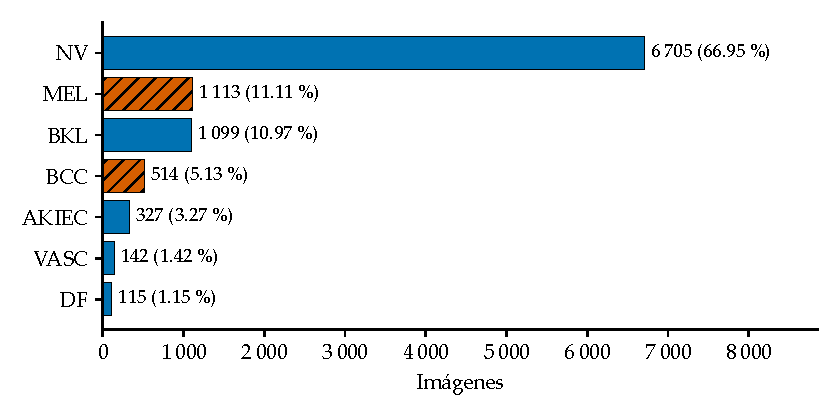
\includegraphics[width=0.8\textwidth]{Figures/Capitulos/03-Materiales-Metodos/ham-distribucion.pdf}
    \caption{Imágenes por clase en \emph{HAM10000} y su porcentaje sobre el total. MEL y BCC en bermellón con trama; las demás clases en azul.}
    \label{fig:met_ham_dist}
\end{figure}

La segunda propiedad afecta a la partición. Una misma lesión puede tener hasta seis imágenes, y las 1\,956 lesiones
con más de una reúnen el 45\,\% del conjunto (Figura~\ref{fig:met_ham_lesiones}). Una situación a evitar es que
imágenes de una misma lesión caigan en entrenamiento y en prueba, ya que el modelo puede reconocer la lesión en lugar
de generalizar a lesiones nuevas, y la prueba deja de medir lo que dice medir. Por eso la partición tiene que agrupar
las imágenes de cada lesión.

\begin{figure}[H]
    \centering
    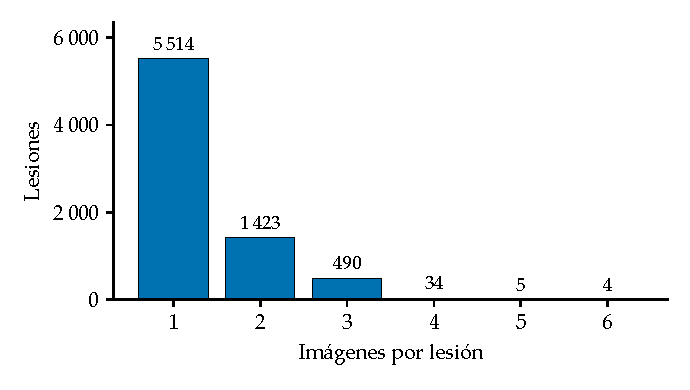
\includegraphics[width=0.7\textwidth]{Figures/Capitulos/03-Materiales-Metodos/ham-imagenes-por-lesion.pdf}
    \caption{Lesiones de \emph{HAM10000} según el número de imágenes que tienen, de una a seis.}
    \label{fig:met_ham_lesiones}
\end{figure}

La tercera propiedad es el respaldo de las etiquetas, que no es el mismo en todas las clases. La histopatología
confirma algo más de la mitad de las imágenes, y todas las de MEL, BCC y AKIEC. En cambio, casi dos tercios de las NV
se confirmaron por seguimiento clínico o por consenso de los autores. La referencia es, por lo tanto, más sólida en
las clases malignas y premalignas que en las benignas. Como ilustración, la Figura~\ref{fig:met_ham_ejemplos} muestra
una imagen de cada clase.

\begin{figure}[H]
    \centering
    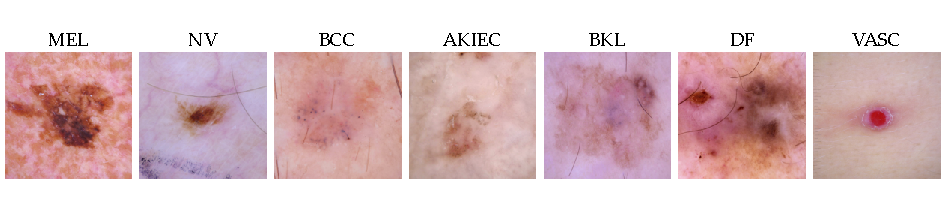
\includegraphics[width=\textwidth]{Figures/Capitulos/03-Materiales-Metodos/ham-ejemplos.pdf}
    \caption{Una imagen dermatoscópica por clase, la primera confirmada por histopatología de cada una. Imágenes de \emph{HAM10000}~\cite{tschandl2018ham10000}, licencia CC BY-NC 4.0. El orden es MEL, NV, BCC, AKIEC, BKL, DF y VASC, las siglas del conjunto.}
    \label{fig:met_ham_ejemplos}
\end{figure}

\subsection{Partición disjunta por lesión}
\label{sec:met_particiones}

La forma habitual de partir un conjunto es asignar cada imagen al azar a una partición, manteniendo en cada una la
proporción de las clases. Con ese procedimiento, una partición frecuente destina el 70\,\% de las imágenes a
entrenamiento, el 15\,\% a validación y el 15\,\% a prueba, y así está construida la partición original de
\emph{HAM10000} con la que comenzó este trabajo. Sin embargo, como la asignación se hace imagen por imagen, dos
imágenes de una misma lesión pueden quedar en particiones distintas. En la partición original, 36 de cada 100
imágenes de prueba tienen otra imagen de su misma lesión en entrenamiento, y entre los melanomas la proporción es de
63 de cada 100.

Esta coincidencia es una fuga de información entre particiones (\emph{data leakage};
Sección~\ref{sec:marco_regularizacion}): el modelo pudo ver en el entrenamiento la misma lesión que se le pide
clasificar, de modo que la prueba ya no mide el desempeño sobre lesiones nuevas. Además, la fuga no afecta a todas las
clases por igual. En NV alcanza al 27\,\% de las imágenes de prueba, mientras que en BCC llega al 70\,\%, así que las
dos clases malignas, que son las que más importan, son las más afectadas.

Para eliminar la fuga, la partición nueva conserva completa la prueba original, de modo que los resultados de los
\glspl{vlm} y del \emph{pipeline}, medidos sobre ella, siguen siendo comparables. Del entrenamiento y la validación
originales se descartan las 776 imágenes cuya lesión aparece en la prueba, y las restantes se reparten con
\texttt{StratifiedGroupKFold} de scikit-learn, con la lesión como grupo, el diagnóstico como estrato y la semilla 42.
Con este procedimiento se obtienen 6\,447 imágenes de entrenamiento y 1\,289 de validación, sin lesiones compartidas entre particiones
(Tabla~\ref{tab:met_tamanos}). El costo es que el entrenamiento tiene un 8\,\% menos de imágenes que el de la partición
original (6\,447 frente a 7\,010). Además, en validación DF y VASC quedan con menos de 20 imágenes, así que sus métricas
por clase en ese conjunto cambian mucho con pocos aciertos.

\begin{table}[H]
    \centering
    \caption{Imágenes por clase y partición de \emph{HAM10000}.}
    \label{tab:met_tamanos}
    \begin{tabularx}{\textwidth}{@{}>{\raggedright\arraybackslash}X r r r r@{}}
        \toprule
        \textbf{Clase} & \textbf{Entrenamiento} & \textbf{Validación} & \textbf{Prueba} & \textbf{Descartadas} \\
        \midrule
        AKIEC & 207 & 41 & 49 & 30 \\
        BCC & 307 & 62 & 77 & 68 \\
        BKL & 682 & 137 & 165 & 115 \\
        DF & 73 & 14 & 17 & 11 \\
        MEL & 661 & 132 & 167 & 153 \\
        NV & 4\,427 & 885 & 1\,006 & 387 \\
        VASC & 90 & 18 & 22 & 12 \\
        \midrule
        \textbf{Total} & \textbf{6\,447} & \textbf{1\,289} & \textbf{1\,503} & \textbf{776} \\
        \bottomrule
    \end{tabularx}
\end{table}

Además de corregirla, interesa saber cuánto sobreestimaba la fuga el desempeño de los clasificadores. Para estimarlo,
el Capítulo~\ref{cp:res_clasif} compara el resultado sobre la prueba completa con el que se obtiene sobre sus 894
imágenes cuya lesión no aparecía ni en entrenamiento ni en validación de la partición original. Como control se usa
DermLIP sin ajuste, que no vio \emph{HAM10000}: si su desempeño también cambia entre ambos conjuntos, el cambio se debe
a la composición del subconjunto y no a la fuga. A diferencia de \emph{HAM10000}, los demás conjuntos no pasan por esta
partición, porque cada uno trae su propia división o se usa completo como prueba.

\subsection{SkinCaRe: SkinCAP y SkinCoT}

En cuanto a la generación de texto, \emph{SkinCaRe} reúne los pares imagen--texto con que se entrenan los generadores
de reportes (Sección~\ref{sec:met_generacion}). Está formado por dos subconjuntos con textos de distinto tipo:
\emph{SkinCAP}, con descripciones escritas por dermatólogos, y \emph{SkinCoT}, con razonamientos diagnósticos.
\emph{SkinCAP} tiene 4\,000 imágenes clínicas tomadas de
\emph{Fitzpatrick 17k} y de \emph{DDI}~\cite{groh2021neural,daneshjou2022disparities}, con descripciones que
escribieron cuatro dermatólogos en chino y que luego se tradujeron al inglés y se revisaron~\cite{shen2025skincare}.
De ellas se excluyen 439 que llevan la marca de descarte que \emph{SKINCON} daba a sus anotadores
para las imágenes de mala calidad~\cite{daneshjou2022skincon}, y las 3\,561 restantes se reparten por imagen con las
mismas proporciones de 70, 15 y 15\,\%.

Por su parte, \emph{SkinCoT} aporta 3\,041 imágenes clínicas del atlas DermNet con un razonamiento diagnóstico escrito para cada
una~\cite{shen2025skincare}. El texto lo produce un modelo de lenguaje que recibe la etiqueta verdadera, y
dermatólogos lo revisan y descartan los de menor puntaje. Como se escribió conociendo el diagnóstico, el razonamiento
muestra cómo se justifica una etiqueta conocida y no cómo se llega a ella desde la imagen, una limitación que pesa al
leer los resultados de generación. Además, el formato intercala bloques \texttt{\textless{}think\textgreater{}} entre
las oraciones y termina con el diagnóstico. Para ilustrarlo, el fragmento siguiente, de un caso de párpados, muestra la
forma; la traducción es propia.

\begin{quote}
    \small
    \texttt{\textless{}think\textgreater{}} First, I observe the primary location: the changes are specifically affecting
    the eyelids (both upper and lower). The skin here is thin and sensitive, making it prone to certain dermatological
    conditions. \texttt{\textless{}/think\textgreater{}}

    \noindent Traducción propia: «Primero, observo la localización principal: los cambios afectan específicamente los
    párpados (superior e inferior). La piel aquí es fina y sensible, lo que la hace propensa a ciertas afecciones
    dermatológicas.»
\end{quote}

\subsection{MM-Skin, HIBA y Derm1M}

A diferencia de \emph{SkinCaRe}, que se usa para entrenar, \emph{MM-Skin} es el conjunto con que se evalúa la
generación contra un texto de referencia. Sus textos son descripciones de quince libros de texto de dermatología,
asociadas a imágenes clínicas, dermatoscópicas y patológicas~\cite{zeng2025mmskin}, y las métricas con referencia se
calculan sobre su partición de prueba (Sección~\ref{sec:met_eval_generacion}). Ninguno de los generadores ajustados en
este trabajo vio \emph{MM-Skin}.
SkinVL, en cambio, sí se ajustó con él y por ello no se evalúa sobre este conjunto.

Por otra parte, \emph{HIBA} reúne 1\,616 imágenes de 623 pacientes de un hospital de Buenos Aires, con licencia CC
BY~\cite{riccilara2023dataset}. Es el único conjunto de otra población y se usa completo como prueba externa, de modo que
ningún modelo se entrena con él (Sección~\ref{sec:marco_generalizacion}). Además, cuatro de cada cinco imágenes son
dermatoscópicas y el resto clínicas, y el melanoma tiene más peso que en \emph{HAM10000} (16\,\% frente a 11\,\%).
Para usarlo con los clasificadores, sus diagnósticos se llevan a las siete categorías de \emph{HAM10000}. En ese
mapeo, el carcinoma escamoso pasa a AKIEC, una aproximación que agrega ruido a la comparación y que se retoma en la
Sección~\ref{sec:met_complementarios}.

Por último, \emph{Derm1M} es el corpus de 1\,029\,761 pares imagen--texto con el que se preentrenó DermLIP~\cite{yan2025derm1miccv}.
Sus imágenes provienen de videos, artículos científicos, foros médicos, conjuntos públicos y material educativo, y sus
textos se limpiaron y resumieron con un \gls{llm}. Entre las fuentes declaradas no figura \emph{HAM10000}, aunque no
puede descartarse que alguna publicación reproduzca imágenes de ese conjunto. El trabajo usa los pesos publicados de
DermLIP sin reentrenarlo, así que \emph{Derm1M} no se usa para entrenar ni para evaluar.

Las características de estos conjuntos orientan la elección de los modelos que se presentan a continuación. Con unas
6\,400 imágenes etiquetadas para siete clases, entrenar un clasificador desde cero no es viable, y por eso los
clasificadores supervisados parten de pesos preentrenados. Por la misma razón, la clasificación con \glspl{vlm} incluye
a DermLIP, que llega preentrenado sobre imágenes de dermatología. Por otra parte, como los textos clínicos disponibles
no usan las siete categorías de \emph{HAM10000}, los generadores aprenden a redactar con \emph{SkinCaRe} y reciben el
diagnóstico de un clasificador, como se describe en la Sección~\ref{sec:met_pipeline}.
